\chapter{Магнетизм атомов. Опыты Штерна и Герлаха. Магнитно-механические 
эффекты. Спин электрона. Квантовые числа электрона и тонкая структура 
спектральных термов. Правила отбора. Понятие об уравнении Дирака.}

Согласно классическим представлениям магнетизм был обусловлен микротоками,
циркулирующими внутри частиц вещества (гипотеза Ампера). Классическая теория не
могла установить природу этих токов, она была отчасти установлена с появлением
электронных представлений о строении вещества (теория Бора). Считалось, что
амперовские токи обусловлены движением электронов внутри атома, однако,
объяснить законы движения этих токов классическая физика не смогла. Кроме того,
методами классической статистической физики было показано, что в установившемся
режиме вещество не может быть намагничено, то есть если намагниченное вещество
предоставить самому себе и поддерживать его температуру постоянной, то оно
самопроизвольно придет в равновесное состояние, в котором намагниченность
отсутствует, даже если вещество помещено в магнитное поле, но это противоречит
опытным фактам.

Понимание природы магнетизма пришло после создания квантовой механики. Магнетизм
является квантовым эффектом.

\begin{minipage}{.27\textwidth}
    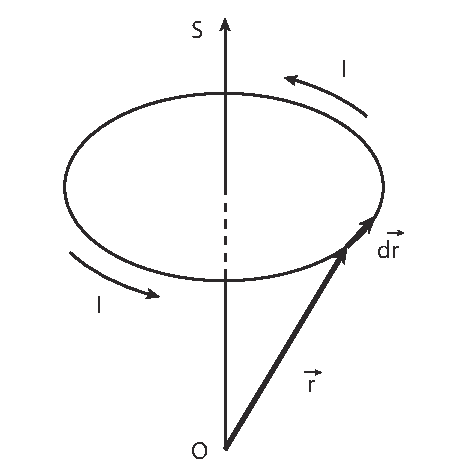
\includegraphics[width=\textwidth]{10_01}
\end{minipage}
\begin{minipage}{.68\textwidth}
    Найдем магнитный момент атома.
    \begin{gather*}
        \vec{M} = I\vec{S}, \quad \vec{S} = \frac{1}{2}\oint [\vec{r}\times\d
        \vec{r}], \quad I = \der{q}{t}, \quad \vec{M} = \frac{1}{2}\oint \der{q}{t}[\vec{r}\times\d\vec{r}] = \\
        = \frac{1}{2}\oint\left[ \vec{r}\times\der{\vec{r}}{t} \right]\,dq =
        \frac{1}{2}\oint[\vec{r}\times\vec{v}]\,dq = \frac{1}{2m}\oint
        [\vec{r}\times\vec{p}]\,dq.
    \end{gather*}

Из последней формулы видно, что из неё выбыло всякое упоминание о витке с
током, осталась лишь система зарядов, каждый из которых характеризуется
положением и скоростью системы.
\end{minipage}

Рассмотрим один заряд: \( \ds \hat{M} = \frac{q}{2m}\left[\hat{\vec{r}}\times
\hat{\vec{p}}\right] \) -- магнитный момент в квантовой механике.

\( \ds \vec{M} = \frac{q}{2m}[\vec{r}\times\vec{p}] = \varGamma\vec{L} \), где
\( \varGamma = q/2m \) -- гиромагнитное отношение. Для электрона: \( \ds \vec{M}
= -\frac{e}{2m_e}\vec{L} \). Модуль магнитного момента может быть определен с
одной из проекций:
\[
    M_z = -\frac{e}{2m_e}L_z = -\frac{e\hbar m}{2m_e} = -\mu_\emph{Б}m, \quad
    \text{где } \mu_\emph{Б} = \frac{e\hbar}{2m_e} \text{ -- магнетон Бора}.
\]

\begin{minipage}{.4\textwidth}
    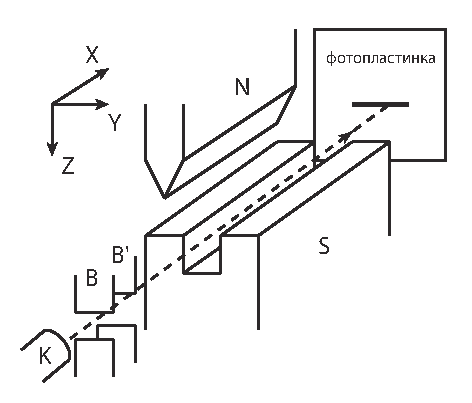
\includegraphics[width=\textwidth]{10_02}
\end{minipage}
\begin{minipage}{.55\textwidth}
    \section{Опыты Штерна и Герлаха}
    Наличие у атомов моментов их квантования было доказано в опытах Штерна и
    Герлаха.

    В сосуде с высоким вакуумом создавался с помощью диафрагм \( B \) и
    \( B' \) атомный пучок исследуемого элемента. Пучок проходил через сильное
    неоднородное магнитное поле \( \vec{H} \), создаваемое особой конструкцией
    магнита. После прохождения через магнитное поле пучок попадал на
    фотопластинку и оставлял на ней след. На атом в неоднородном магнитном поле
    действует сила:
\end{minipage}
\[
    \vec{f} = (\vec{M}\vec{\nabla})\vec{B}, \quad f_z = M_x\pder{B_x}{x} +
    M_y\pder{B_y}{y} + M_z\pder{B_z}{z} = M_z\pder{B_z}{z}.
\]

\section{Магнито-механические эффекты}
Результаты опытов Эйнштейна и де Гааза, а также опытов Барнета по определению
гиромагнитного отношения показали, что, например, для железа гиромагнитное
отношение вдвое больше, чем требуется по теории. Квантовая теория на тот момент
не могла объяснить тонкую структуру щелочных металлов.

Для описания этой структуры трех квантовых чисел \( n,\,l,\,m \) оказалось
недостаточно. Уленбек и Гаудсмит выдвинули гипотезу о спине электрона: электрон
имеет не только момент количества движения и магнитный момент, связанные с
движением частицы, как целого, но и собственный механический момент количества
движения. Этот собственный механический момент называется спином.

\section{Квантовые числа электрона и тонкая структура спектральных термов}
В квантовой механике состояние электрона описывается четырьмя квантовыми
числами: главным квантовым числом \( n \), орбитальным квантовым числом \( l \),
орбитальным магнитным квантовым числом \( m_l \), спиновым квантовым числом
\( m_s \). Спиновое число \( m_s \) определяет проекцию вектора спина
\( \vec{s} \) на выделенное направление. Спин \( \vec{s} \) может быть
ориентирован либо по \( \vec{l} \), либо против \( \vec{l} \), то есть проекция
может принимать только два значения: \( \ds L_{z_s} = \pm\frac{\hbar}{2} \).
Орбитальный момент количества движения \( \vec{l} \) и спиновый момент
\( \vec{s} \) складываются в полный момент количества движения: \( \vec{j} =
\vec{l} + \vec{s} \), его проекция: \( \ds m_j = m_l + m_s = m_l \pm\frac{1}{2}
\).

Тонкая структура обусловлена спин-орбитальным взаимодействием, само же СОВ
обусловлено взаимодействием между спином электрона и зарядом ядра.

\section{Наглядное физическое истолкование СОВ}
Воспользуемся теорией Бора для атома водорода: электрон, вращаясь по орбите,
обладает спиновым магнитным моментом. Электрическое поле ядра оказывает
воздействие на спиновый магнитный момент \( M_{z_s} \) может принимать только 2
возможных ориентации в пространстве, вдоль и против магнитного момента. Поэтому
из-за СОВ каждый энергетический уровень атома щелочного металла распадается на 2
состояния, за исключением \( S \) состояния.

В квантовой механике доказывается правило отбора для полного квантового числа
\( j \): \( \Delta j = 0,\, \pm 1 \).

\section{Понятие об уравнении Дирака}
 
Релятивистское волновое уравнение должно быть:
\begin{enumerate}
    \item инвариантно по отношению к преобразованиям Лоренца;
    \item линейно, чтобы выполнялся принцип суперпозиции для волновых функций;
    \item симметрично (т.е. содержать первые производные);
    \item из него должно вытекать соотношение полной энергии \( E^2 = m^2c^4 +
p^2c^2 \).
\end{enumerate}

Чтобы удовлетворять всем требованиям, волновая функция должна быть
многокомпонентной, в случае электрона компонент четыре:
\[
    \psi = \begin{bmatrix} \psi_1 \\ \psi_2 \\ \psi_3 \\ \psi_4 \end{bmatrix}.
\]

Имеем систему уравнений:
\[
    \left\{ \begin{array}{l}
        \ds \i\hbar\pder{\psi_1}{t} = mc^2\psi_1 + c(\hat{p}_x - \i\hat{p}_y)
        \psi_4 + c\hat{p}_z\psi_3, \\[.4em]
        \ds \i\hbar\pder{\psi_2}{t} = mc^2\psi_2 + c(\hat{p}_x + \i\hat{p}_y)
        \psi_3 - c\hat{p}_z\psi_4, \\[.4em]
        \ds \i\hbar\pder{\psi_3}{t} = -mc^2\psi_3 + c(\hat{p}_x - \i\hat{p}_y)
        \psi_2 + c\hat{p}_z\psi_1, \\[.4em]
        \ds \i\hbar\pder{\psi_4}{t} = -mc^2\psi_4 + c(\hat{p}_x + \i\hat{p}_y)
        \psi_1 - c\hat{p}_z\psi_2,
    \end{array} \right.
\]
где \( \ds \hat{p}_{x_k} = -\i\hbar\pder{}{x_k} \).

Следствия из уравнения Дирака:
\begin{enumerate}
    \item электрон должен обладать собственным механическим моментом импульса --
    спином;
    
    \item энергия может быть как положительной, так и отрицательной: \( E^2 =
    m^2c^4 + p^2c^2 \). Отсюда следует, что для частиц существуют античастицы --
    с одинаковой массой, но противоположным по знаку зарядом;
    
    \item тонкая структура атома водорода выражается следующей формулой:
    \[
        E_H = -\frac{m_e}{2}\left(\frac{kZe^2}{\hbar}\right)^2 \frac{1}{n^2}
        \left[1 + \frac{(\alpha kZ)^2}{n}\left(\frac{1}{j + \frac{1}{2}} -
        \frac{3}{4n}\right)\right].
    \]
\end{enumerate}

\newpage
